\section{Why the analogies hold: reduced-order models}
\label{sec:reduced}

Engineers often understand a complex system through a simple model that shares its governing terms. Sloshing in a partially filled liquid tank is a free-surface flow, yet its response regimes, including the strongly nonlinear ones with hydraulic impacts on the walls, are reproduced by an equivalent mechanical model in which a linear oscillator is coupled to a vibro-impact unit \citep{farid2017response}. Section~\ref{sec:dictionary} showed that the clocks and textbook physical systems behave alike. This section explains why, with reductions of the same kind. For each one we name the physical model and its governing equation (Figure~\ref{fig:models}), derive the part of the language model that reduces to it, and state where the reduction stops holding. Table~\ref{tab:reduced} summarizes the six cases, and the subsections follow its order: three results on clock~3, two on clock~2 and one on clock~1.

\begin{table}[t]
\centering
\small
\caption{Reduced-order models of language-model behavior. The shared term is the part of the governing equation that produces the behavior in both systems.}
\label{tab:reduced}
\begin{tabular}{p{0.2\linewidth}p{0.22\linewidth}p{0.26\linewidth}p{0.21\linewidth}}
\toprule
Language model & Reduced model & Shared term & Status \\
\midrule
Escape from a loop (clock 3) & Particle in a well under noise, Fig.~\ref{fig:models}(b) & Boltzmann factor: $e^{-\Delta/T}$ and $e^{-\Delta U/D}$ & Exact identity (Prop.~\ref{prop:arrhenius}) \\
Loops that hold for a while (clock 3) & Particle in a deepening well, Fig.~\ref{fig:models}(d) & Barrier that grows with residence time & Fitted; $T_{1/2}$ within 9\% to 25\% \\
Regimes of generation (clock 3) & Noisy double-well Duffing oscillator, Fig.~\ref{fig:models}(a) & Ratio of barrier to noise & Same ordering, measured \\
Period two at the edge of stability (clock 2) & Explicit Euler step on a nonlinear spring & Step multiplier $1-\eta\lambda$ crossing $-1$, cubic term of the loss & Derived; multi-mode edge not covered \\
Loss spike (clock 2) & Ball in a valley whose stiffness changes along it, Fig.~\ref{fig:catapult} & Step multiplier $1-\eta\lambda$ below $-1$ where the valley is stiff & Exact for the two-parameter model; untested at scale \\
Clustering over depth (clock 1) & Kuramoto oscillators, Fig.~\ref{fig:models}(c) & Coupling $\sin(\psi_j-\psi_i)$ & Exact for idealized attention; trained GPT-2 departs \\
\bottomrule
\end{tabular}
\end{table}

\subsection{Escape from a loop: the softmax is a Boltzmann distribution}
\label{sec:loops}

Repetition loops are the case where the reduction is exact, so we start with the noise-driven escape of Section~\ref{sec:escape}.

\paragraph{The softmax is a Boltzmann distribution.} In statistical mechanics a system in contact with a heat bath occupies a state of energy $E$ with probability proportional to $e^{-E/k_BT}$. The sampler \eqref{eq:clock3} has exactly this form, with the energy of token $y$ equal to minus its logit, $E_y=-z_y$, and $k_B=1$. A token is a state, a logit is minus an energy, and the sampling temperature is a temperature in the physical sense. Suppose the chain has entered a loop of period $k$ with tokens $a_1,\dots,a_k$. As long as the sampler keeps choosing the loop token, the context is deterministic, so the logits $z_i$ at the $i$-th step of the loop are fixed numbers. The loop token $a_i$ has the highest logit, and every other token $y$ is an exit whose energy is higher by the logit gap $\Delta_i^{y}=z_i(a_i)-z_i(y)>0$. The probability of staying in the loop at step $i$ is
\begin{equation}
p_i(T)=\frac{1}{1+S_i(T)},\qquad S_i(T)=\sum_{y\neq a_i} e^{-\Delta_i^{y}/T},
\label{eq:stay}
\end{equation}
and the probability of leaving during one cycle is $r(T)=1-\prod_{i=1}^{k}p_i(T)$ (Figure~\ref{fig:models}b). At low temperature the probability of leaving at step $i$ is
\begin{equation}
1-p_i(T)=\frac{S_i(T)}{1+S_i(T)}\;\approx\;m_i\,e^{-\Delta_i/T}\qquad (T\to0),
\label{eq:boltz_exit}
\end{equation}
where $\Delta_i$ is the smallest gap and $m_i$ the number of tokens that attain it. This is the Arrhenius factor of Kramers' problem \eqref{eq:kramers}, with the logit gap in place of the barrier height $\Delta U$ and $T$ in place of the noise intensity $D$ (Figure~\ref{fig:models}b). The correspondence is an identity, which is why every loop in Figure~\ref{fig:pair_escape}(b) gives a straight line whose slope is its gap. Two differences remain. A Brownian particle diffuses up to the barrier, and the curvatures at the bottom and the top of the well set Kramers' prefactor; the sampler jumps in one step, so the prefactor is the number of exits $m_i$. In addition, the energies of a language model change as the context grows, which Section~\ref{sec:deepening} treats.



\begin{proposition}[Arrhenius law for loop escape]
\label{prop:arrhenius}
Let $\Delta_{\min}=\min_i\min_{y\neq a_i}\Delta_i^{y}$ and let $m$ be the number of pairs $(i,y)$ that attain it. Then $r(T)\le \sum_{i}S_i(T)$ for all $T>0$, and
\begin{equation}
r(T)= m\, e^{-\Delta_{\min}/T}\,\big(1+o(1)\big)\quad\text{as } T\to0,\qquad\text{so}\qquad \lim_{T\to0}T\log r(T)=-\Delta_{\min}.
\end{equation}
\end{proposition}
\noindent The proof is in Appendix~\ref{app:proofs}.

The logit gap therefore plays the role of the barrier height $\Delta U$ in Kramers' formula \citep{kramers1940brownian}, and $T$ plays the role of noise intensity. Proposition~\ref{prop:arrhenius} follows almost directly from the Gibbs form of the softmax. \citet{chen2026repetition} use the same product of per-step continuation probabilities to ask when a sampler locks a loop exactly, with probability one, and show that plain temperature sampling never does. Here a loop locks in a weaker, probabilistic sense: the probability of never escaping is positive (Proposition~\ref{prop:lock}), or escape takes longer than the generation (Section~\ref{sec:exp3}).

\subsection{Loops that hold for a while: a well that deepens while it is occupied}
\label{sec:deepening}

The Boltzmann identity \eqref{eq:boltz_exit} holds at every step, but the energies change from cycle to cycle, because each completed cycle adds the same text to the context and the model grows more confident that it will repeat it, the self-reinforcement reported by \citet{xu2022learning}. Figure~\ref{fig:reduced}(a) shows the smallest gap $\Delta_c$ of each cycle along three GPT-2 loops: it grows and then saturates. The physical counterpart is a particle in a well that deepens while it is occupied (Figure~\ref{fig:models}d). Rock friction behaves this way: the static friction between two surfaces grows with the time they have been in contact \citep{dieterich1972time}, so a block that has rested longer needs a larger force to slide.

To see what this growth does to escape, let $\Delta_c$ be the smallest gap during cycle $c$ and $r_c(T)$ the escape probability during that cycle. The probability of never leaving is $\prod_{c\ge1}(1-r_c(T))$, which is positive exactly when $\sum_c r_c(T)<\infty$ (given $r_c<1$).

\begin{proposition}[Deepening wells lock]
\label{prop:lock}
If $\Delta_c\ge\Delta_1+b\,(c-1)$ for some $b>0$, then for every $T>0$ the probability of never escaping is at least $1-k(|\mathcal V|-1)\,e^{-\Delta_1/T}/(1-e^{-b/T})$ whenever this bound is positive, and the probability itself is positive for every $T>0$. If instead the logits along the loop converge from cycle to cycle, so that $\Delta_c\to\Delta_\infty<\infty$, escape eventually happens with probability one, but the expected number of cycles before escape grows like $e^{\Delta_\infty/T}$ as $T\to0$.
\end{proposition}
\noindent The proof is in Appendix~\ref{app:proofs}.

Between linear growth and saturation lies a growth law with a sharp threshold in temperature.

\begin{proposition}[Locking temperature]
\label{prop:tlock}
If $\Delta_c=\Delta_1+\gamma\ln c$ for all $c\ge1$ with $\gamma>0$, the probability of never escaping is positive for $T<\gamma$, and escape happens with probability one for $T\ge\gamma$. For $T>\gamma$ the probability of staying in the loop for $N$ cycles is $\exp\!\big(-\Theta(N^{1-\gamma/T})\big)$.
\end{proposition}
\noindent The proof is in Appendix~\ref{app:proofs}.

Proposition~\ref{prop:tlock} gives an infinite-horizon locking temperature $T_{\mathrm{lock}}=\gamma$, below which survival decays to a positive constant and above which it decays as a stretched exponential. Linear growth locks at every temperature and saturating growth at none, so the three cases of Propositions~\ref{prop:lock} and \ref{prop:tlock} cover the possible outcomes for an unbounded generation. A real generation has a finite budget of $N$ cycles. If the barrier has saturated at $\Delta_\infty$ and the escape probability per cycle is $m\,e^{-\Delta_\infty/T}\ll1$, survival over $N$ cycles equals one half at
\begin{equation}
T_{1/2}(N)\approx\frac{\Delta_\infty}{\ln\!\big(mN/\ln2\big)},
\label{eq:thalf}
\end{equation}
so the locking temperature observed in a saturating loop falls like $1/\ln N$ with the length of the generation. In practice logits are bounded, so the gaps cannot grow without limit. Experiment~3 (Section~\ref{sec:exp3}) measures $\Delta_c$ along real loops of GPT-2 and Pythia, tests Propositions~\ref{prop:arrhenius} and \ref{prop:lock} against the exact survival probabilities and against Monte Carlo sampling, and finds that the barriers saturate. A reduced model with a saturating barrier is therefore the right one for real loops.

\paragraph{A reduced model for real loops.} The reduced model has two ingredients, a saturating barrier fitted to the gaps of each loop,
\begin{equation}
\Delta_c=\Delta_\infty-(\Delta_\infty-\Delta_1)\,e^{-(c-1)/c_\ast},\qquad r_c(T)=1-\big(1+e^{-\Delta_c/T}\big)^{-\nu},
\label{eq:reduced}
\end{equation}
and an escape probability per cycle $r_c$ for a single exit attempted $\nu$ times per cycle. The three numbers $\Delta_1,\Delta_\infty,c_\ast$ of each loop come from its greedy run alone, and $\nu$ plays the role of Kramers' prefactor; we use one value per model, chosen on a grid ($\nu=3$ for GPT-2, $\nu=4$ for Pythia-160M). Figure~\ref{fig:reduced} compares the locking temperature $T_{1/2}(N)$ of this model with the full computation from all logits of all steps (Section~\ref{sec:exp3}). For horizons of 4 to 256 cycles the reduced model is within a median of 9\% to 25\% of the full value for individual loops, with correlations of 0.74 to 0.95 across loops, and it reproduces the slow fall of $T_{1/2}$ with $N$. For a single cycle it is off by 30\% to 50\%. For long horizons the reduced model gives $T_{1/2}(N)\approx\Delta_\infty/\ln(\nu N/\ln2)$, the form of \eqref{eq:thalf}, since an escape within $N$ cycles becomes likely once $\nu N e^{-\Delta_\infty/T}$ is of order one, so the locking temperature falls like $1/\ln N$.

\begin{figure}[t]
\centering
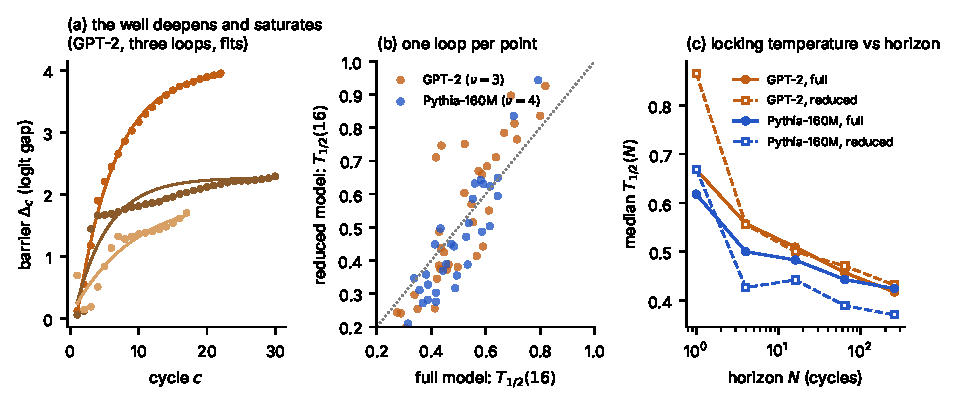
\includegraphics[width=\textwidth]{figs/reduced.pdf}
\caption{The reduced-order model of loop escape against the full computation. (a) Smallest logit gap of each cycle (dots) along three GPT-2 loops of at least 15 cycles, with the saturating fit of \eqref{eq:reduced} (lines). (b) Locking temperature for a horizon of 16 cycles after a burn-in of two cycles, from the reduced model (three numbers per loop read from the greedy run, one attempt number $\nu$ per model) against the full computation from all logits, one point per loop. (c) Median locking temperature against the horizon for both models, full (filled) and reduced (open).}
\label{fig:reduced}
\end{figure}

\subsection{One number orders the regimes of generation}
\label{sec:collapse}

The Boltzmann identity also accounts for the regimes of Section~\ref{sec:regimes}. If escape from a well is governed by the factor $e^{-\text{barrier}/\text{noise}}$, the motion of a system with wells is organized by one dimensionless number, the ratio of barrier height to noise intensity, whatever the other details of the system. The prediction is that the oscillator and the language model of Figure~\ref{fig:atlas} leave their periodic orbits at the same value of this ratio, a value set by the length of the observation. For the double-well Duffing oscillator with unit mass, friction coefficient $\zeta$ and noise term $\sqrt{2\zeta D}\,\xi$, the unforced motion has the stationary density $\propto\exp\{-(\dot q^2/2+U(q))/D\}$, so the depth of a well in units of the noise is $\Delta U/D$, with $\Delta U=1/4$ for $U=-q^2/2+q^4/4$. If an escape has probability of order $e^{-\Delta U/D}$ per period, the oscillator is expected to leave a well within $N$ periods once $\Delta U/D\lesssim\ln(N/\ln2)$. Above this value it stays on a periodic orbit in one well, close to it the oscillator hops between wells, and far below it the noise dominates. For a loop of a language model the corresponding ratio is $\Delta/T$, with $\Delta$ the barrier of the loop, and the same estimate gives $\Delta/T\lesssim\ln(\nu N/\ln2)$, with $N$ the number of cycles in the window. Figure~\ref{fig:collapse} plots the determinism of the trajectory against this ratio for both systems. For the oscillator (512 samples, about 98 forcing periods, so $\ln(N/\ln2)\approx4.9$) DET rises from 0.38 to 0.78 as $\Delta U/D$ grows from 0.09 to 50, with its largest step between 3.1 and 5.6. For GPT-2 we sampled five prompts whose greedy runs loop, at eight temperatures from 0.3 to 1.4, and took $\Delta$ as the gap of the last cycles of the greedy loop. DET rises with $\Delta/T$ (correlation 0.75 with $\log(\Delta/T)$ over 40 runs), and the binned median climbs from 0.37 to 0.82 between $\Delta/T\approx5.6$ and 12, just above the value 4.9 at which one escape is expected in the window. The scatter between prompts is large, and five prompts do not determine the shape of the curve, but both systems leave the periodic regime when the barrier falls to a few times the noise, at the value set by the length of the observation.

\begin{figure}[t]
\centering
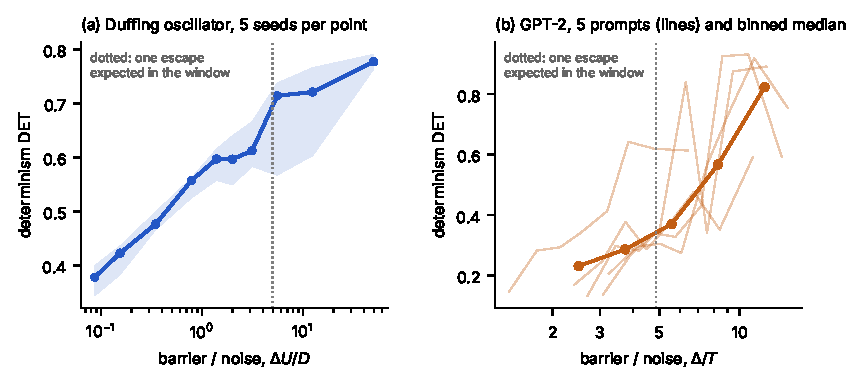
\includegraphics[width=0.85\textwidth]{figs/collapse.pdf}
\caption{Determinism of the trajectory against the ratio of barrier height to noise intensity. (a) Forced double-well Duffing oscillator of Figure~\ref{fig:atlas}, ten noise levels, five seeds each (median and range), with $\Delta U=1/4$. (b) GPT-2, five prompts whose greedy runs end in a loop, sampled at eight temperatures from 0.3 to 1.4; $\Delta$ is the median logit gap of the last three cycles of the greedy loop. Thin lines: individual prompts; thick line: median in bins of $\Delta/T$. Dotted lines: the ratio at which one escape is expected within the observed window, $\ln(N/\ln2)$ for the oscillator and $\ln(\nu N/\ln2)$ with $\nu=3$ for GPT-2.}
\label{fig:collapse}
\end{figure}

\subsection{The edge of stability: an Euler step on a nonlinear spring}
\label{sec:spring}

We now turn to clock~2. The edge of stability of Section~\ref{sec:eos}, where training settles on a period-2 orbit at the threshold $2/\eta$, has a reduction that takes one line. Gradient descent $\theta_{t+1}=\theta_t-\eta\nabla\mathcal L(\theta_t)$ is the explicit Euler scheme with step $\eta$ for the gradient flow $\dot\theta=-\nabla\mathcal L(\theta)$, the motion of an overdamped particle in the potential $\mathcal L$. Restrict it to the eigenvector $v$ of the largest Hessian eigenvalue $\lambda$ at a minimum $\theta^\ast$, with $q=\langle\theta-\theta^\ast,v\rangle$ and $\mathcal L_v(q)=\mathcal L(\theta^\ast+qv)$. Then
\begin{equation}
q_{t+1}=q_t-\eta\,\mathcal L_v'(q_t),\qquad \mathcal L_v'(q)=\lambda q+\tfrac12\mathcal L_v'''q^2+\tfrac16\mathcal L_v''''q^3+\dots,
\label{eq:gd_spring}
\end{equation}
and $-\mathcal L_v'(q)$ is the restoring force of a spring with linear, quadratic and cubic stiffness, the Duffing spring of Figure~\ref{fig:models}(a) when the quadratic term vanishes. The linear term alone gives $q_{t+1}=(1-\eta\lambda)q_t$, whose multiplier crosses $-1$ at $\eta\lambda=2$. The minimum then loses stability through a period-doubling bifurcation, the same instability that limits the time step of the explicit Euler scheme for a stiff spring. The nonlinear terms decide what follows. For the double well $\mathcal L_v(q)=(q^2-1)^2/4$ around $q=1$, where $\lambda=2$, the iterate settles on a period-2 orbit for $\eta\lambda$ between 2 and about 2.47, on a period-4 orbit from 2.48, on a period-8 orbit near 2.58, and on no orbit of period up to 64 from about 2.62 (Figure~\ref{fig:pair_training}a,b). A period-2 orbit is what produces the spectral line at frequency $1/2$.

\paragraph{A spring whose stiffness responds to the motion.} A network adds a third ingredient: $\lambda$ depends on $\theta$, so the oscillation along $v$ changes the curvature that drives it, and the motion and the stiffness are coupled. \citet{damian2022selfstabilization} reduce this feedback to a two-variable map. With $q_t$ the displacement along the top eigenvector $v$ and $\lambda_t$ the sharpness, linearized around a point where it equals $2/\eta$, the two evolve as
\begin{equation}
q_{t+1}=(1-\eta\lambda_t)\,q_t,\qquad \lambda_{t+1}=\lambda_t+\eta\big(\alpha-\|\nabla\lambda_{\max}\|^2 q_t^2\big),
\label{eq:selfstab}
\end{equation}
where $\alpha>0$ measures progressive sharpening and the cubic term of the loss enters through the gradient of the sharpness, $\nabla\lambda_{\max}$. The first equation is the linear step of \eqref{eq:gd_spring} with a stiffness that now moves. The oscillation grows while $\eta\lambda_t>2$, and its square pulls $\lambda_t$ back, so the pair cycles around the threshold instead of diverging. Mechanically, this is a mass in an elastic well whose walls soften when the mass swings hard, an oscillator whose stiffness is a slow variable driven by the amplitude of the motion. The feedback explains why the transformer of Experiment~2 shows a line at $1/2$ (Figure~\ref{fig:pair_training}c,f) across two decades of step size instead of a cascade to chaos at one step size: training keeps its own bifurcation parameter at the threshold. The one-direction reduction holds while one eigenvalue dominates. In our transformer two to six eigenvalues sit above $2/\eta$ (Section~\ref{sec:exp2}), which neither \eqref{eq:gd_spring} nor the two-variable map describes. Related results include conditions under which gradient descent converges while being locally unstable \citep{arora2022gradient,ahn2022unstable}, solvable minimal models with edge-of-stability dynamics \citep{zhu2022edgeofstability}, convergence to stable period-two orbits beyond the threshold, a period-doubling bifurcation in the strict sense \citep{chen2022edge}, and the implicit penalty on the gradient norm that backward error analysis finds in the finite step \citep{barrett2020implicit}.

\subsection{A loss spike: a ball thrown out of a stiff valley}
\label{sec:catapult}

The same instability, seen in a loss landscape whose stiffness changes from place to place, produces loss spikes. Large pretraining runs show such spikes. PaLM handled them by restarting from an earlier checkpoint and skipping data \citep{chowdhery2022palm}. \citet{wortsman2023smallscale} reproduced two instability mechanisms at small scale, growth of attention logits and divergence of the output logits, and studied how they depend on learning rate. Attention entropy collapse is another proposed cause \citep{zhai2023stabilizing}, as is the behavior of the Adam update at large scale \citep{molybog2023theory}; conditions on the scale of embeddings and residual connections can prevent spikes \citep{takase2023spike}. The smallest model with a loss spike has two parameters, and it shows the mechanism in a form that can be drawn.

In the catapult model of \citet{lewkowycz2020large} the product $w_1w_2$ of two scalar weights is fit to a single target with step size $\eta$. The loss $(w_1w_2-1)^2/2$ has a valley of minima along the hyperbola $w_1w_2=1$, and the curvature across the valley at $(w_1,w_2)$ is $w_1^2+w_2^2$, large far out along the axes and smallest at $w_1=w_2=1$ (Figure~\ref{fig:catapult}a). The mechanical picture is a ball moved by the explicit Euler steps of Section~\ref{sec:spring} in a channel whose walls are steep at one end and gentle at the other. Started on the steep part, where $\eta(w_1^2+w_2^2)>2$, each step overshoots the floor and the ball bounces from wall to wall with growing amplitude, the period-doubling instability of \eqref{eq:gd_spring}: the loss spikes. The bouncing also carries the ball along the channel toward the gentle end, and once it reaches the part where $\eta(w_1^2+w_2^2)<2$, the steps stop overshooting and the ball settles on the floor. With $\eta=0.95$ the loss rises tenfold within two steps and the iterate settles where the curvature, 2.01, is below $2/\eta=2.11$ (Figure~\ref{fig:catapult}b,c). \citet{lewkowycz2020large} call this the catapult phase; above a second threshold training diverges, and \citet{kalra2023phase} mapped these early-training regimes as a function of learning rate, depth and width. Whether the spikes of large pretraining runs are catapults, crossings of the stability boundary or escapes from a basin is open (\op{4}).

\begin{figure}[t]
\centering
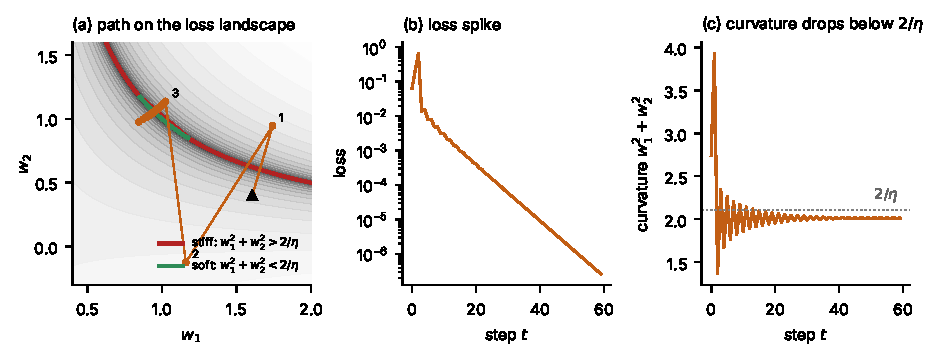
\includegraphics[width=\textwidth]{figs/catapult.pdf}
\caption{A loss spike in two parameters, seen as a ball thrown out of a stiff valley. Gradient descent on $(w_1w_2-1)^2/2$ with $\eta=0.95$, started near $(w_1,w_2)=(1.6,0.4)$ where the curvature across the valley of minima, $w_1^2+w_2^2=2.74$, exceeds $2/\eta=2.11$. (a) Path of the iterate (triangle: start; numbers: the first three steps) on the loss landscape (gray: log loss); the valley of minima $w_1w_2=1$ is red where it is too stiff for the step size and green where it is not. (b) The loss jumps from 0.064 to 0.66 and then decays. (c) The curvature oscillates and settles at 2.01, below $2/\eta$.}
\label{fig:catapult}
\end{figure}

\subsection{Clustering over depth: attention on the circle is a Kuramoto model}
\label{sec:kuramoto}

The last reduction concerns clock~1 and explains the synchronization of Section~\ref{sec:particles}. In the transformer model of \citet{geshkovski2023mathematical}, layer normalization keeps every token on the unit sphere, and self-attention with identity query, key and value matrices moves token $i$ by
\begin{equation*}
\dot x_i=\Pi_{x_i}\Big(Z_i^{-1}\sum_j e^{\beta\langle x_i,x_j\rangle}x_j\Big),\qquad Z_i=\sum_j e^{\beta\langle x_i,x_j\rangle},
\end{equation*}
where $\Pi_x$ projects onto the tangent space of the sphere at $x$. In two dimensions write $x_i=(\cos\psi_i,\sin\psi_i)$. The unit tangent at $x_i$ is $(-\sin\psi_i,\cos\psi_i)$, its inner product with $x_j$ is $\sin(\psi_j-\psi_i)$, and $\langle x_i,x_j\rangle=\cos(\psi_j-\psi_i)$, so
\begin{equation}
\dot\psi_i=Z_i^{-1}\sum_j e^{\beta\cos(\psi_j-\psi_i)}\sin(\psi_j-\psi_i).
\label{eq:attn_kuramoto}
\end{equation}
For $\beta=0$, $Z_i=n$ and \eqref{eq:attn_kuramoto} is the Kuramoto model \eqref{eq:kuramoto} with $\omega_i=0$ and $J=1$, the model of identical metronomes on a common board, which synchronize from almost every initial condition (Figure~\ref{fig:models}c). In both systems each unit is pulled toward a weighted average of the others, and for $\beta>0$ the pull is stronger between tokens that are already close, which lets several clusters form and persist (Section~\ref{sec:particles}). The reduction accounts for Figure~\ref{fig:pair_depth}(c) and for GPT-2 with random weights in panel (d). Trained GPT-2 departs from it: its order parameter stays near 0.8 over all twelve blocks. The reduction drops the learned query, key and value maps, the MLP blocks and the finite depth. One candidate explanation is that these terms act like the spread of natural frequencies $\omega_i$ in the Kuramoto model, which opposes synchronization; we have not tested it.
